\begin{frame}
\frametitle{Ghost Values}

\begin{block}{To evaluate a local function $f(x)$, each process requires}
\begin{itemize}
  \item its local portion of the vector $x$
  \item its {\color{cyan}ghost values}, bordering portions of $x$ owned by neighboring processes
\end{itemize}
\end{block}

\begin{center}
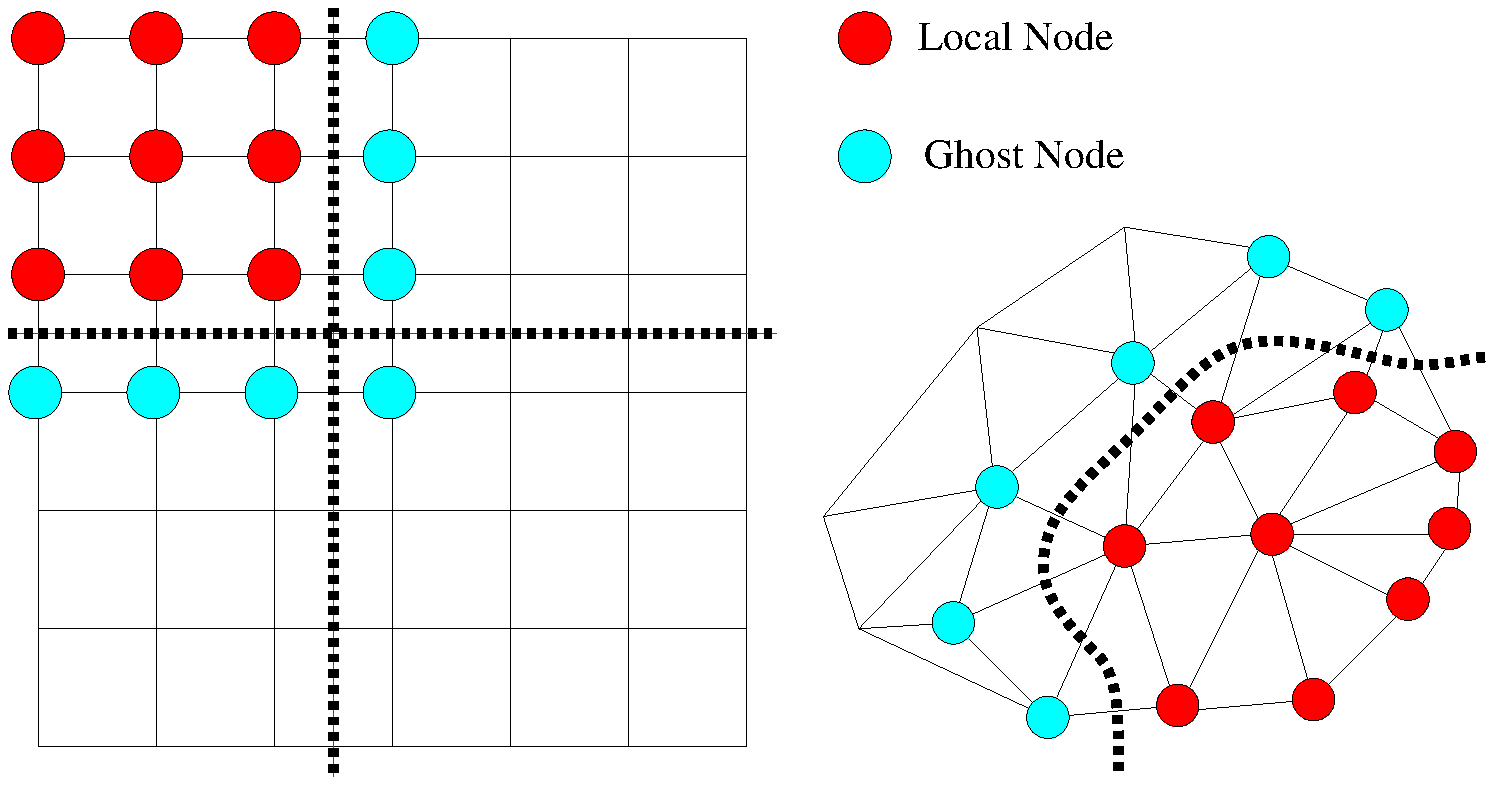
\includegraphics[width=4in]{figures/GhostValues}
\end{center}

\end{frame}
